\let\negmedspace\undefined
\let\negthickspace\undefined
\documentclass[journal]{IEEEtran}
\usepackage[a5paper, margin=10mm, onecolumn]{geometry}
%\usepackage{lmodern} % Ensure lmodern is loaded for pdflatex
\usepackage{tfrupee} % Include tfrupee package

\setlength{\headheight}{1cm} % Set the height of the header box
\setlength{\headsep}{0mm}     % Set the distance between the header box and the top of the text

\usepackage{gvv-book}
\usepackage{gvv}
\usepackage{cite}
\usepackage{amsmath,amssymb,amsfonts,amsthm}
\usepackage{algorithmic}
\usepackage{graphicx}
\usepackage{textcomp}
\usepackage{xcolor}
\usepackage{txfonts}
\usepackage{listings}
\usepackage{enumitem}
\usepackage{mathtools}
\usepackage{gensymb}
\usepackage{comment}
\usepackage[breaklinks=true]{hyperref}
\usepackage{tkz-euclide} 
\usepackage{listings}
% \usepackage{gvv}                                        
\def\inputGnumericTable{}                                 
\usepackage[latin1]{inputenc}                                
\usepackage{color}                                            
\usepackage{array}                                            
\usepackage{longtable}                                       
\usepackage{calc}                                             
\usepackage{multirow}                                         
\usepackage{hhline}                                           
\usepackage{ifthen}                                           
\usepackage{lscape}
\usepackage{circuitikz}


\renewcommand{\thefigure}{\theenumi}
\renewcommand{\thetable}{\theenumi}
\setlength{\intextsep}{10pt} % Space between text and floats


\numberwithin{equation}{enumi}
\numberwithin{figure}{enumi}
\renewcommand{\thetable}{\theenumi}


% Marks the beginning of the document
\begin{document}
\bibliographystyle{IEEEtran}
\vspace{3cm}

\title{GATE 2018}
\author{EE25BTECH11065 - YOSHITA.J}
\maketitle

% (add your content here)
\noindent \textbf{Q. 1 -- Q. \textbf{5}} carry one mark each.

\begin{enumerate}
    \item ``Going by the\rule{3cm}{0.15mm} that many hands make light work, the school\rule{3cm}{0.15mm} involved all the students in the task"\\The word that best fills the blank in the above sentence is
    \begin{multicols}{2}
    \begin{enumerate}
        \item  principle, principal
        \item  principal, principle\\
        \item  principle, principle
        \item  principal, principal
    \end{enumerate}
    \end{multicols}
    \hfill{$\brak{ GATE\ EY\ 2018}$}
    \bigskip
    \item ``Her\rule{3cm}{0.15mm} should not be confused with miserliness; she is ever willing to assist those on need."\\The word that best fills the blank in the above sentence is
\begin{multicols}{4}
\begin{enumerate}
    \item cleanliness
    \item punctuality
    \item frugality
    \item greatness
\end{enumerate}
\end{multicols}
\hfill{$\brak{ GATE\ EY\ 2018}$}
\bigskip
\item Seven machines take 7 minutes to make 7 identical toys. At the same rate, how many minutes would it take for 100 machines to make 100 toys?
\begin{multicols}{4}
\begin{enumerate}
    \item $1$
    \item $7$
    \item $100$
    \item $700$
\end{enumerate}
\end{multicols}
\hfill{$\brak{ GATE\ EY\ 2018}$}
\bigskip
\item A rectangle becomes a square when its length and breadth are reduced by 10 m and 5 m, respectively. During this process, the rectangle loses 650 $m^2$ of area. What is the area of the original rectangle in square meters?
\begin{multicols}{4}
\begin{enumerate}
    \item $1125$
    \item $2250$
    \item $2924$
    \item $4500$
\end{enumerate}
\end{multicols}
\hfill{$\brak{ GATE\ EY\ 2018}$}
\bigskip
\item A number consists of two digits. The sum of digits is $9$. If $45$ is subtracted from the number, its digits are interchanged. What is the number?
\begin{multicols}{4}
\begin{enumerate}
    \item $63$
    \item $72$
    \item $81$
    \item $90$
\end{enumerate}
\end{multicols}
\hfill{$\brak{ GATE\ EY\ 2018}$}
\bigskip
\\
\noindent \textbf{Q. 6 -- Q. \textbf{10}} carry one mark each.
\\
\item For integers a, b and c, what would be the minimum and maximum values respectively of $a+b+c$ if $\log|a|+\log|b|+\log|c|=0$?
\begin{multicols}{4}
\begin{enumerate}
    \item $-3$ and $3$
    \item $-1$ and $1$
    \item $-1$ and $3$
    \item $1$ and $3$
\end{enumerate}
\end{multicols}
\hfill{$\brak{ GATE\ EY\ 2018}$}
\bigskip
 \item Given that $a$ and $b$ are integers and $a+a^2b^3$ is odd, which one of the following statements is correct?
\begin{multicols}{2}
\begin{enumerate}
    \item $a$ and $b$ are both odd
    \item $a$ and $b$ are both even
    \item $a$ is even and $b$ is odd
    \item $a$ is odd and $b$ is even
\end{enumerate}
\end{multicols}
\hfill{$\brak{ GATE\ EY\ 2018}$}
\bigskip
\item From the time the front of a train enters a platform, it takes $25$ seconds for the back of the train to leave the platform, while traveling at a constant speed of $54$ km/h. At the same speed, it takes $14$ seconds to pass a man running at $9$ km/h in the same direction as the train. What is the length of the train and that of the platform in meters, respectively?
\begin{multicols}{2}
\begin{enumerate}
    \item $210$ and $140$
    \item $162.5$ and $187.5$
    \item $245$ and $130$
    \item $175$ and $200$
\end{enumerate}
\end{multicols}
\hfill{$\brak{ GATE\ EY\ 2018}$}
\bigskip
\item Which of the following functions describe the graph shown in the below figure?
\begin{figure}[H]
    \centering
    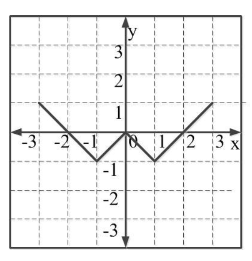
\includegraphics[width=0.5\columnwidth]{figs/9.png}
    \caption{}
    \label{fig:9}
   \end{figure}
\begin{multicols}{2}
\begin{enumerate}
    \item $y = ||x|+1|-2$ 
    \item $y = ||x|-1|-1$
    \item $y = ||x|+1|-1|$
    \item $y = ||x-1|-1|$
\end{enumerate}
\end{multicols}
\hfill{$\brak{ GATE\ EY\ 2018}$}
\bigskip
\item Consider the following three statements:\\$\brak{i}$ Some roses are red.\\$\brak{ii}$ All red flowers fade quickly.\\$\brak{iii}$ Some roses fade quickly.\\Which of the following statement can be logically inferred from the above statements?
\begin{enumerate}
    \item If $\brak{i}$ is true and $\brak{ii}$ is false, then $\brak{iii}$is false.
    \item If $\brak{i}$ is true and $\brak{ii}$ is false, then $\brak{iii}$ is true.
    \item If $\brak{i}$ and $\brak{ii}$ are true, then $\brak{iii}$ is true.
    \item If $\brak{i}$ and $\brak{ii}$ are false, then $\brak{iii}$ is false.
\end{enumerate}
\hfill{$\brak{ GATE\ EY\ 2018}$}
\begin{center}
\Large
\textbf{END OF THE QUESTION PAPER}
\end{center}
\end{enumerate}

\newpage
\noindent \textbf{Q. 1 -- Q. \textbf{25}} carry one mark each.\\
\begin{enumerate}

\item During the Pleistocene, which of the following groups experienced the largest mass extinction?
    \begin{enumerate}
        \item Large dinosaurs
        \item Large mammals
        \item Reptiles
        \item Trilobites
    \end{enumerate}
    \hfill{$\brak{ GATE\ EY\ 2018}$}
    \bigskip
\item In gropu living species, the term ``dilution effect" refers to
    \begin{enumerate}
        \item reduction in aggression among individuals with increasing group size
        \item reduction in the mobility of individuals with increasing group size
        \item reduction in the reproductive success of individuals with increasing group size
        \item reduction in the risk of predation with increasing group size
    \end{enumerate}
    \hfill{$\brak{ GATE\ EY\ 2018}$}
    \bigskip
\item Which of the following diversity indices best captures species turnover across habitats?
\begin{multicols}{4}
    \begin{enumerate}
        \item $\alpha$
        \item $\beta$
        \item $\gamma$
        \item $\delta$
    \end{enumerate}
    \end{multicols}
    \hfill{$\brak{ GATE\ EY\ 2018}$}
    \bigskip
\item A duck egg is removed from its mother's nest and incubated by a barnyard hen. The
duckling hatches out in the presence of the barnyard hen and stays in her nest. After
a couple of days, the duckling is presented with a choice between its biological
mother and the hen that incubated it. The duckling approaches and follows the hen.
This set of observations demonstrates the phenomenon of
    \begin{enumerate}
        \item habituation
        \item imprinting
        \item instinct
        \item sensitization
    \end{enumerate}
    \hfill{$\brak{ GATE\ EY\ 2018}$}
    \bigskip
\item If both of your ears were located next to each other in the middle of your face, you
would have difficulty in resolving the
    \begin{enumerate}
        \item direction of a sound
        \item duration of a sound
        \item loudness of a sound 
        \item pitch of a sound
    \end{enumerate}
    \hfill{$\brak{ GATE\ EY\ 2018}$}
    \bigskip
\item Forager bees communicate the distance of a food source using a waggle dance upon
return to the hive. It is observed that the number of waggles of a dance increases
linearly with the distance to the food source. This tells us that the
    \begin{enumerate}
        \item number of waggles and distance to food source is negatively correlated
        \item  number of waggles and distance to food source is positively correlated
        \item number of waggles affects the distance to the food source
        \item number of waggles and the distance to the food source are uncorrelated
    \end{enumerate}
    \hfill{$\brak{ GATE\ EY\ 2018}$}
    \bigskip
\item Male frogs display to females by producing loud acoustic signals. The use of these
signals by bats to locate frogs and prey upon them is an example of
    \begin{enumerate}
        \item aposematism
        \item deception
        \item eavesdropping
        \item mimicry
    \end{enumerate}
    \hfill{$\brak{ GATE\ EY\ 2018}$}
    \bigskip
\item A non-venomous, non-toxic species of snake is brightly colored and closely
resembles a venomous snake species in the same habitat. This is most likely a case
of
    \begin{enumerate}
        \item aggressive mimicry
        \item batesian mimicry
        \item masquerade
        \item mullerian mimicry
    \end{enumerate}
    \hfill{$\brak{ GATE\ EY\ 2018}$}
    \bigskip
\item The value of the resting membrane potential of a typical neuron is closest to the
equilibrium potential of which of the following ions?
\begin{multicols}{4}
    \begin{enumerate}
        \item $Ca^{++}$
        \item $K^+$
        \item $Mg^{++}$
        \item $Na^+$
    \end{enumerate}
    \end{multicols}
    \hfill{$\brak{ GATE\ EY\ 2018}$}
    \bigskip
\item A plant species found in India produces flowers that are white, fragrant, and tubular.
Which of the following is the most likely pollinating agent?
\begin{multicols}{2}
    \begin{enumerate}
        \item Hummingbirds
        \item Lorises
        \item Moths
        \item Wind    
    \end{enumerate}
    \end{multicols}
    \hfill{$\brak{ GATE\ EY\ 2018}$}
    \bigskip
\item Which of the following can be used to test differences between mean tree heights in
a tropical versus a temperate forest?
    \begin{enumerate}
        \item Binomial test
        \item Linear regression
        \item Pearson's correlation
        \item Student's t-test
    \end{enumerate}
    \hfill{$\brak{ GATE\ EY\ 2018}$}
    \bigskip
\item For a species, assuming a relatively short tome scale and no evolution, increased interspecific competition will result in a 
\begin{multicols}{2}
    \begin{enumerate}
        \item larger fundamental niche
        \item larger realized niche
        \item smaller fundamental niche
        \item smaller realized niche
    \end{enumerate}
    \end{multicols}
    \hfill{$\brak{ GATE\ EY\ 2018}$}
    \bigskip
\item In which of the following mating systems is sperm competition likely to evolve?
    \begin{enumerate}
        \item Monoandry
        \item Monogamy
        \item Polyandry
        \item Polygyny
    \end{enumerate}
    \hfill{$\brak{ GATE\ EY\ 2018}$}
    \bigskip
\item Copies of genes that arrive in a particular genome by horizontal gene transfer are
known as
\begin{multicols}{4}
    \begin{enumerate}
        \item analogs
        \item homologs
        \item ohnologs
        \item xenologs
    \end{enumerate}
    \end{multicols}
    \hfill{$\brak{ GATE\ EY\ 2018}$}
    \bigskip
\item In which of the following plants is the dominant stage of the life cycle haploid?
\begin{multicols}{2}
    \begin{enumerate}
        \item Cycads
        \item Ferns
        \item Gymnosperms
        \item Mosses
    \end{enumerate}
    \end{multicols}
    \hfill{$\brak{ GATE\ EY\ 2018}$}
    \bigskip
\item Which of the following is NOT typically a characteristic of carly successional
pioneer plants relative to late successional plants in a tropical rain forest?
\begin{multicols}{2}
    \begin{enumerate}
        \item Higher shade tolerance
        \item Smaller seed size
        \item Smaller size at maturity
        \item Wind dispersed seeds
    \end{enumerate}
    \end{multicols}
    \hfill{$\brak{ GATE\ EY\ 2018}$}
    \bigskip
\item Natural populations often deviate from Hardy-Weinberg equilibrium. One possible
reason for this is
\begin{multicols}{2}
    \begin{enumerate}
        \item no migration
        \item no selection
        \item random mating
        \item small population sizes
    \end{enumerate}
    \end{multicols}
    \hfill{$\brak{ GATE\ EY\ 2018}$}
    \bigskip
\item Which of the following is NOT an example of phenotypic plasticity?
    \begin{enumerate}
        \item Density-dependent swarming behavior in locusts
        \item Increase in DDT resistance in mosquitos
        \item Seasonal variation in plumage coloration in birds 
        \item Temperature-dependent sex determination in turtles
    \end{enumerate}
    \hfill{$\brak{ GATE\ EY\ 2018}$}
    \bigskip
\item Which of the following is NOT a characteristic of r-selected species?
    \begin{enumerate}
        \item Early sexual maturity
        \item High juvenile mortality
        \item High parental care
        \item Large number of offspring
    \end{enumerate}
    \hfill{$\brak{ GATE\ EY\ 2018}$}
    \bigskip
\item A scientist finds a new species of insect and sends a sample to a museum for
confirmation. The curator of the museum designates it as a holotype for the newly
identified species and asks the scientist to also provide samples of the opposite sex.
This sample of the opposite sex is called the
\begin{multicols}{4}
    \begin{enumerate}
        \item allotype
        \item isotype
        \item karyotype
        \item neotype
    \end{enumerate}
    \end{multicols}
    \hfill{$\brak{ GATE\ EY\ 2018}$}
    \bigskip
\item Which of the following is NOT essential for a behavioural trait to evolve by natural
selection?
    \begin{enumerate}
        \item The behavioral trait differs among individuals
        \item The behavioral trait is determined at least in part by genes
        \item The behavioral trait influences reproductive success
        \item The behavioral trait is determined entirely by genes
    \end{enumerate}
    \hfill{$\brak{ GATE\ EY\ 2018}$}
    \bigskip
\item El Nino Southern Oscillation $\brak{ENSO}$ events have occurred approximately every
3-7 years over the last century. The cause of these ENSO events is related to
    \begin{enumerate}
        \item large-scale air-sea interactions in the Pacific Ocean
        \item strong monsoon winds in the Indian Ocean
        \item the melting of icebergs in the Antarctic Ocean
        \item unsustainable overfishing in North Atlantic Ocean
    \end{enumerate}
    \hfill{$\brak{ GATE\ EY\ 2018}$}
    \bigskip
\item If the mean of a sample is $5$, and the variance is $25$, the PERCENT coefficient of
variation is

    \hfill{$\brak{ GATE\ EY\ 2018}$}
    \bigskip
\item Consider a diploid population at Hardy-Weinberg equilibrium. For a locus with two
alleles, the frequency of the $A_1A_2$ genotype is $0.01$. The frequency of heterozygotes $A_1A_2$ is\rule{3cm}{0.15mm}
$\brak{answer\ up\ to\ 2\ decimal\ places}$
   
    \hfill{$\brak{ GATE\ EY\ 2018}$}
    \bigskip
\item In a food chain, the efficiency of transfer of energy from one trophic level to the
next is $10\%$. The PERCENTAGE of energy that is expected to transfer from the
second to the fourth level is\rule{3cm}{0.15mm}.

    \hfill{$\brak{ GATE\ EY\ 2018}$}
    \bigskip
\\
\noindent \textbf{Q. 26 -- Q. \textbf{55}} carry one mark each.
\\
\item Which of the following is an adaptation for osmoregulation in freshwater teleost
fish?
    \begin{enumerate}
        \item Excreting large quantities of dilute urine
        \item Excreting large quantities of uric acid
        \item Having high concentration of blood urea
        \item Excreting large quantities of uracil
    \end{enumerate}
    \hfill{$\brak{ GATE\ EY\ 2018}$}
    \bigskip
\item The latitudinal diversity gradient is defined as the decrease in the number of species
from the equator to the poles. This can result from
    \begin{enumerate}
        \item greater energy input at the poles
        \item greater land mass at the poles
        \item greater seasonal variation at the poles
        \item greater speciation rates at the poles 
    \end{enumerate}
    \hfill{$\brak{ GATE\ EY\ 2018}$}
    \bigskip
\item Identify the graph in which natural selection on beak size is LEAST likely to be
occurring? For each of the graphs, the slope of the regression line and the associated
p-value is given.\\
\begin{figure}[!ht]
\centering
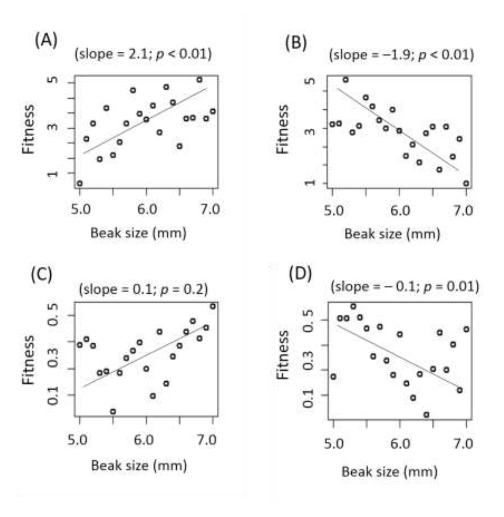
\includegraphics[width=0.26\columnwidth]{figs/1.png}
\label{fig:1}
\end{figure}

    \hfill{$\brak{ GATE\ EY\ 2018}$}
    \bigskip
\item Some species of spiders add additional silk `decorations' to their webs. It is
hypothesized that these decorations serve either to lure flies $\brak{prey}$ or to decrease
bird $\brak{predator}$ attacks on the spiders. The appropriate way to test these hypotheses
would be to compare numbers of
    \begin{enumerate}
        \item predators and prey approaching decorated webs
        \item  predators and prey approaching undecorated webs 
        \item predators approaching decorated webs with prey approaching undecorated webs 
        \item  predators and prey approaching both decorated and undecorated webs
    \end{enumerate}
    \hfill{$\brak{ GATE\ EY\ 2018}$}
    \bigskip
\item The figure below shows mean annual temperatures (\textcelsius) and mean annual
precipitation $\brak{cm\ per\ year}$ from multiple sites in four regions in India.
\begin{figure}[!ht]
    \centering
    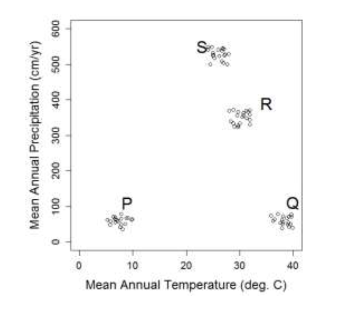
\includegraphics[width=0.5\columnwidth]{figs/5.png}
    \caption{}
    \label{fig:5}
   \end{figure}
    \begin{enumerate}
        \item P:Andaman, Q:Meghalaya, R:Ladakh, S:Rajasthan
        \item P:Ladakh, Q:Rajasthan, R:Andaman, S:Meghalaya
        \item P:Meghalaya, Q:Ladakh, R:Rajasthan, S:Andaman
        \item P:Rajasthan, Q:Andaman, R:Meghalaya, S:Ladakh
    \end{enumerate}
    \hfill{$\brak{ GATE\ EY\ 2018}$}
    \bigskip
\item For a pair of interacting species, increased specialization and decreased niche
breadth in both species would result in
    \begin{enumerate}
        \item decreased intraspecific competition and increased interspecific competition
        \item decreased intraspecific competition and decreased interspecific competition
        \item increased intraspecific competition and increased interspecific competition
        \item increased intraspecific competition and decreased interspecific competition
    \end{enumerate}
    \hfill{$\brak{ GATE\ EY\ 2018}$}
    \bigskip
    \item Males of a bird species provide parental care by feeding nestlings before they
fledge. Which of the following is a PROXIMATE explanation for this behaviour?
    \begin{enumerate}
        \item Feeding nestlings increases their survivorship after fledging
        \item High prolactin levels cause males to feed their nestlings
        \item Males from all species in this genus provide parental care
        \item Males that provide parental care have higher fitness
    \end{enumerate}
    \hfill{$\brak{ GATE\ EY\ 2018}$}
    \bigskip
\item The courtship display of a spider species consists of both visual and vibrational
signals. Females respond to the display by approaching males. In an experiment,
females were presented with $3$ treatments: i) only videos of displaying males, ii)
only vibrational signals of the display, and iii) both videos of displaying males and
vibrational signals. The results are given below: 
\begin{figure}[!ht]
    \centering
    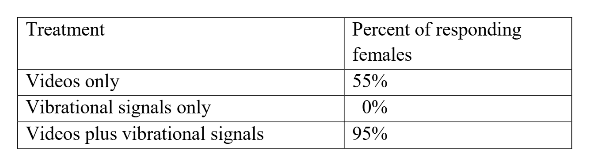
\includegraphics[width=0.6\columnwidth]{figs/2.png}
    \caption{}
    \label{fig:2}
   \end{figure}
   \\
   Results from this experiment show that 
    \begin{enumerate}
        \item vibrational signals are necessary to evoke a response
        \item vibrational signals are sufficient to evoke a response
        \item visual and vibrational signals are necessary to evoke a response
        \item visual signals are necessary to evoke a response
    \end{enumerate}
    \hfill{$\brak{ GATE\ EY\ 2018}$}
    \bigskip
    \item Moth cars typically consist of a membranous cardrum backed by an air cavity. Ears
in different phylogenetic groups of moths have evolved on different body parts.
Moth ears are thus best described as
    \begin{enumerate}
        \item convergent organs
        \item homologous organs
        \item maladaptive organs
        \item vestigcal organs
    \end{enumerate}
    \hfill{$\brak{ GATE\ EY\ 2018}$}
    \bigskip
    \item Increased anthropogenic disturbance has resulted in an overall decrease in densities
of trees and an increase in fragmentation of forests. Which of the following types of
trees will have the greatest reduction in reproductive success?
    \begin{enumerate}
        \item Dioecious species
        \item Monoceious species
        \item Self-compatible hermaphrodites
        \item Self-incompatible hermaphrodites
    \end{enumerate}
    \hfill{$\brak{ GATE\ EY\ 2018}$}
    \bigskip
    \item A study examined the effect of neighbours on plants when grown at low or high
altitudes. The researcher measured Relative Neighbour Effect $\brak{RNE}$, defined as:
RNE = Biomass with neighbours - Biomass without neighbours.
\begin{figure}[!ht]
    \centering
    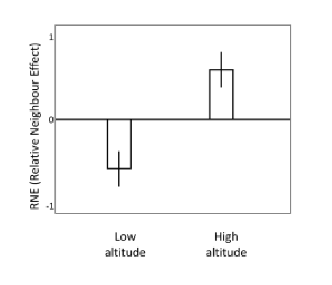
\includegraphics[width=0.5\columnwidth]{figs/3.png}
    \caption{}
    \label{fig:3}
   \end{figure}
    \begin{enumerate}
        \item competition at both altitudes
        \item competition at high altitudes, and facilitation at low altitudes
        \item competition at low altitudes, and facilitation at high altitudes
        \item facilitation at both altitudes
    \end{enumerate}
    \hfill{$\brak{ GATE\ EY\ 2018}$}
    \bigskip
    \item Match the combination of flora and fauna from the list, to the state where they are
found.
\begin{figure}[!ht]
    \centering
    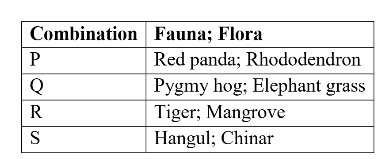
\includegraphics[width=0.5\columnwidth]{figs/4.png}
    \caption{}
    \label{fig:4}
   \end{figure}
    \begin{enumerate}
        \item P:Assam, Q:Jammu \& Kashmir, R:West bengal, S:Sikkim
        \item P:Jammu \& Kashmir, Q:Assam, R:West bengal, S:Sikkim
        \item P:Sikkim, Q:Assam, R:West bengal, S:Jammu \& kashmir
        \item P:Sikkim, Q:West bengal, R:Assam, S:Jammu \& Kashmir
    \end{enumerate}
    \hfill{$\brak{ GATE\ EY\ 2018}$}
    \bigskip
    \item A parent population $\brak{P}$ is split into three daughter populations $\brak{Q, R, and S}$ which
grow in three different habitats. After $1000$ generations, the equilibrium frequency
distribution of a trait in each of the daughter populations is shown in the figure
below. For reference, the vertical line represents the mean of the parent population.
\begin{figure}[!ht]
    \centering
    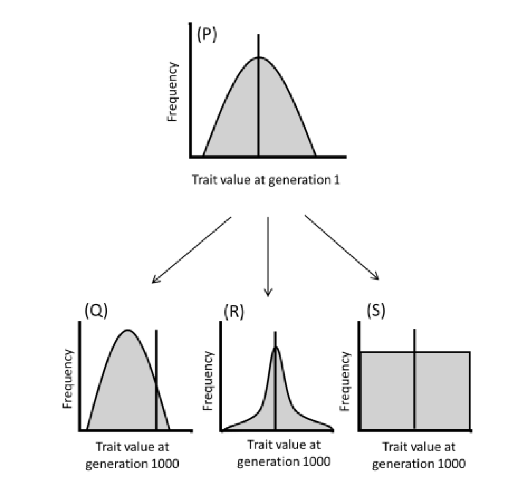
\includegraphics[width=0.6\columnwidth]{figs/6.png}
    \caption{}
    \label{fig:6}
   \end{figure}
   From this information, one can infer that the subpopulations experienced the
following selection regimes
\begin{enumerate}
        \item Q: Directional; R: Stabilizing; S: No selection
        \item Q: Directional; R: Stabilizing; S: Stabilizing
        \item Q: Directional; R: Directional; S: Stabilizing
        \item Q: Stabilizing; R: Directional; S: No selection
    \end{enumerate}
    \hfill{$\brak{ GATE\ EY\ 2018}$}
    \bigskip
    \item The character matrix below lists four taxa $brak{P-S}$ and their nine characters $brak{i-ix}$. A
character state is designated as `0' if it is ancestral and `$1$' if it is derived. Which of
the following phylogenetic trees is obtained by cladistic analysis of these data?
    \begin{figure}[!ht]
    \centering
    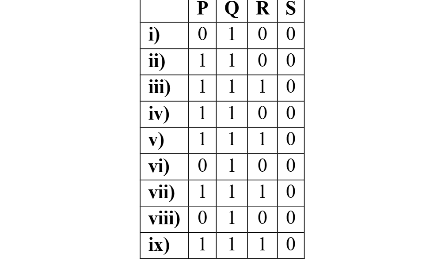
\includegraphics[width=0.2\columnwidth]{figs/7.png}
    \caption{}
    \label{fig:7}
   \end{figure}
   \begin{figure}[!ht]
    \centering
    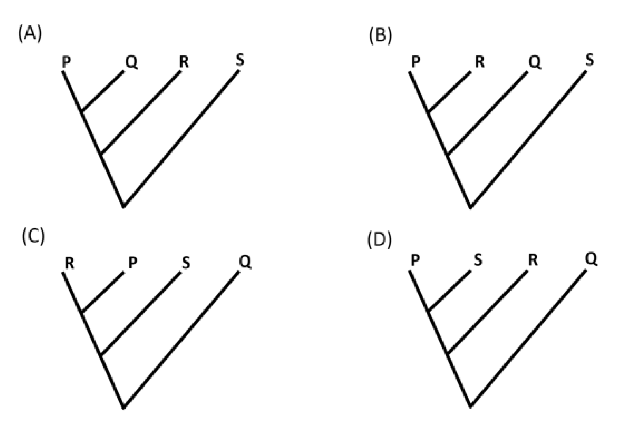
\includegraphics[width=0.3\columnwidth]{figs/17.png}
    \caption{}
    \label{fig:17}
   \end{figure}
   \\
    \hfill{$\brak{ GATE\ EY\ 2018}$}
    \bigskip
    
\item The reactions below $\brak{R1\ and\ R2}$ represent different carbon fixation pathways in
photosynthesis.

RuBP represents Ribulose bisphosphate.
Rubisco represents RuBP carboxylase-oxygenase.
PGA represents Phosphoglyceric acid.
PEP represents Phosphocnolpyruvate.
\begin{figure}[!ht]
    \centering
    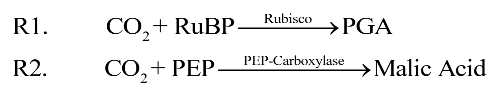
\includegraphics[width=0.5\columnwidth]{figs/8.png}
    \caption{}
    \label{fig:8}
   \end{figure}
   Which of the following is CORRECT?
    \begin{enumerate}
        \item R$1$ and R$2$ both occur in C-$3$ and CAM photosynthesis
        \item R$1$ occurs in C-$4$ photosynthesis; R$2$ occurs in C-$3$ photosynthesis
        \item R$1$ occurs in C-$3$ photosynthesis; R$2$ occurs in C-$4$ photosynthesis
        \item R$l$ occurs in C-$4$ and CAM photosynthesis; R$2$ occurs in C-$3$ photosynthesis
    \end{enumerate}
    \hfill{$\brak{ GATE\ EY\ 2018}$}
    \bigskip
    \item A fish species is sexually dimorphic: males possess ultraviolet $\brak{UV}$ spots on their
bodies which are lacking in females. Females prefer males with larger and more
intense UV spots as mates. Which of the following statements is a plausible reason
for the spots being colored ultraviolet?
    \begin{enumerate}
        \item Females assess males from long distances
        \item Females are not sensitive to UV light 
        \item Ultraviolet spots are a poor indicator of male quality
        \item Ultraviolet spots are more conspicuous to predators
    \end{enumerate}
    \hfill{$\brak{ GATE\ EY\ 2018}$}
    \bigskip
    \item A climate scientist notices a trend in atmospheric $CO2$ concentrations $\brak{in\ ppm}$ at a
research station. Although overall $CO2$ is rising over decades, there are intra-annual
fluctuations, as shown in the figure below.
   \begin{figure}[!ht]
    \centering
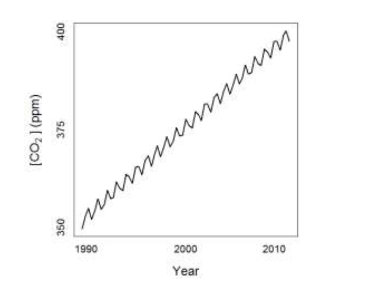
\includegraphics[width=0.3\columnwidth]{figs/10.png}
    \caption{}
    \label{fig:10}
   \end{figure}
   These fluctuations can be attributed to\\
   \\
    \begin{enumerate}
        \item burning of fossil fuels by automobiles and industry
        \item oscillations due to El Nino and La Nina events
        \item rising sea levels due to melting of polar ice-caps
        \item seasonal trends in photosynthesis and respiration
    \end{enumerate}
    \hfill{$\brak{ GATE\ EY\ 2018}$}
    \bigskip
\item Four islands differ in size $\brak{small = 10 km^2,\ large = 100 km^2}$ and distance from the
mainland $\brak{near\ =\ 50 km,\ far\ =\ 500\ km}$.
Island P is small and near the mainland;
Island Q is small and far from the mainland;
Island R is large and near the mainland;
Island S is large and far from the mainland
\\
Let $N_p$, $N_Q$, $N_R$ and $N_s$ denote the number of species on islands P, Q, R and S,
respectively. Which of the following is consistent with the theory of island
biogcography?
\begin{multicols}{2}
    \begin{enumerate}
        \item $N_Q>N_s > N_p> N_R$
        \item $N_R>N_Q>N_p>N_s$
        \item $N_Q>N_p>N_s>N_R$
        \item $N_R> N_p > N_s > N_Q$
    \end{enumerate}
    \end{multicols}
    \hfill{$\brak{ GATE\ EY\ 2018}$}
    \bigskip
\item The rate of population growth $(\frac{dN}{dt})$ over time $\brak{t}$ is shown below
\begin{figure}[!ht]
    \centering
    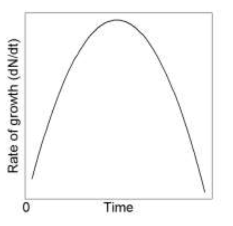
\includegraphics[width=0.3\columnwidth]{figs/11.png}
    \caption{}
    \label{fig:11}
   \end{figure}\\
   For the above population, which of the following plots of population $\brak{Popn.}$ size $\brak{N}$ vs. time $\brak{t}$ is CORRECT?
    \begin{figure}[!ht]
    \centering
    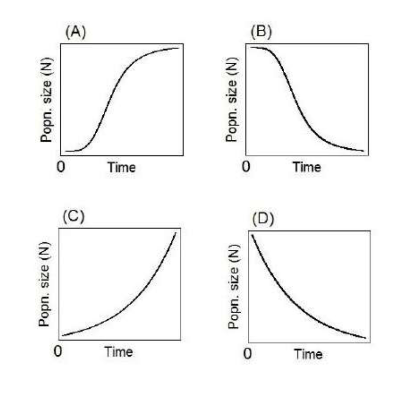
\includegraphics[width=0.4\columnwidth]{figs/12.png}
    \caption{}
    \label{fig:12}
   \end{figure}
    \hfill{$\brak{ GATE\ EY\ 2018}$}
    \bigskip
\item The pedigree below details a late onset genetic disease among humans. Males are
represented as squares and females as circles. Individuals with the disease arc
depicted as black, and those without it are depicted as white. Which of the following
best describes the pattern of inheritance of the disease-causing gene?
\begin{figure}[!ht]
    \centering
    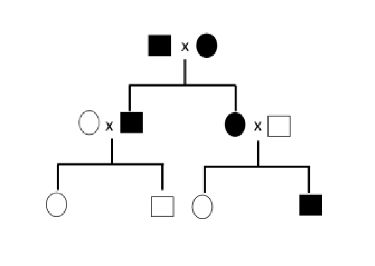
\includegraphics[width=\linewidth]{figs/13.png}
    \caption{}
    \label{fig:13}
   \end{figure}
    \begin{enumerate}
        \item Mitochondrial
        \item X-linked dominant
        \item X-linked recessive
        \item Y-linked
    \end{enumerate}
    \hfill{$\brak{ GATE\ EY\ 2018}$}
    \bigskip
\item Match the following scientists with the concepts or theories they are associated
with.
\begin{figure}[!ht]
    \centering
    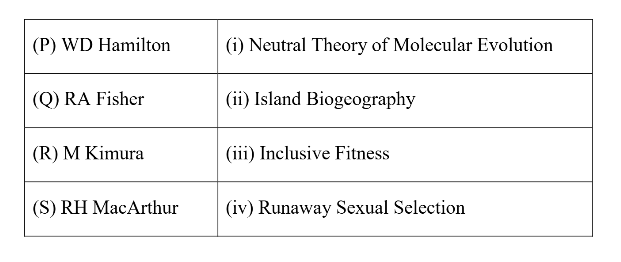
\includegraphics[width=\linewidth]{figs/14.png}
    \caption{}
    \label{fig:14}
   \end{figure}
    \begin{enumerate}
        \item P-iii, Q-i, R-iv, S-ii
        \item P-ii, Q-iii, R-iv, S-i
        \item P-iii, Q-iv, R-i, S-ii
        \item P-ii, Q-iii, R-i, S-iv
    \end{enumerate}
    \hfill{$\brak{ GATE\ EY\ 2018}$}
    \bigskip
\item Which of the following is an example of complete intrinsic post-zygotic
reproductive isolation between two species P and Q?
    \begin{enumerate}
        \item P and Q can mate and have fertile offspring
        \item P and Q can mate but their offspring are inviable
        \item P and Q have breeding seasons during different times of the year
        \item P and Q have different courtship behaviour
    \end{enumerate}
    \hfill{$\brak{ GATE\ EY\ 2018}$}
    \bigskip
\item Match the animals to their locomotor adaptation
\begin{figure}[!ht]
    \centering
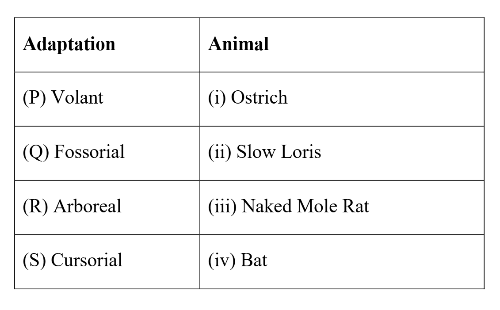
\includegraphics[width=0.5\columnwidth]{figs/15.png}
    \caption{}
    \label{fig:15}
   \end{figure}
\\
   \begin{multicols}{2}
    \begin{enumerate}
        \item P-iv, Q-i, R-iii, S-ii
        \item P-iv, Q-iii, R-ii, S-i
        \item P-iii, Q-iv, R-i, S-ii
        \item P-ii, Q-iii, R-i, S-ii
    \end{enumerate}
    \end{multicols}
    \hfill{$\brak{ GATE\ EY\ 2018}$}
    \bigskip
\item Paralogs are genes that are the products of gene duplication events within a species.
Orthologs are genes in different species that share a common ancestral gene. The
figure below describes the evolutionary history of a hypothetical gene X in
organism Y. This gene undergoes a duplication event. Later, Y splits into two
species $Y_1$ and $Y_2$, and this gives rise to four copies of the gene - P, Q, R and S.
Which option best describes the relationships between the four copies of the
gene X?
\begin{figure}[!ht]
    \centering
    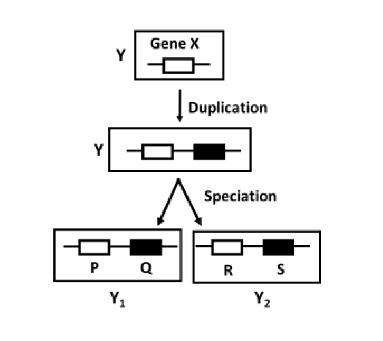
\includegraphics[width=0.5\columnwidth]{figs/16.png}
    \caption{}
    \label{fig:16}
   \end{figure}
    \begin{enumerate}
        \item P \& Q are orthologs, Q \& R are paralogs
        \item R \& S are orthologs, S \& Q are paralogs
        \item R \& S are orthologs, Q \& R are paralogs
        \item P \& R are orthologs, R \& S are paralogs
    \end{enumerate}
    \hfill{$\brak{ GATE\ EY\ 2018}$}
    \bigskip
\item The frequency distribution of beak sizes of a bird species is symmetric but not
normally distributed. If the mean value of beak size is $6$ mm, standard deviation is
$25$ mm and kurtosis is $10$, then the median is\rule{3cm}{0.15mm} mm.\\
   
    \hfill{$\brak{ GATE\ EY\ 2018}$}
    \bigskip
\item An altruist provides help worth $10$ units of fitness to a recipient, at a personal cost of
$1$ unit of fitness. As per kin-selection theory, the minimum value of genetic
relatedness between the actors and the recipients that is necessary to maintain
altruism in the population is\rule{3cm}{0.15mm} $\brak{answer\ up\ to\ 1\ decimal\ place}$.\\
   
    \hfill{$\brak{ GATE\ EY\ 2018}$}
    \bigskip
   \item A population grows from a size of $100$ individuals at t = $0$, to $1000$ individuals at
t = $100$, following density-independent growth. The ratio of per-capita growth rates
at the initial $\brak{at\ t=0}$ to the final $\brak{t=100}$ time is\rule{3cm}{0.15mm}\\
   
    \hfill{$\brak{ GATE\ EY\ 2018}$}
    \bigskip
\item The probability that a bush has a cricket is $0.1$. The probability of a spider being
present on a bush is $0.2$. When both a spider and a cricket are present on a bush, the
probability of encountering each other is $0.2$. The probability of a spider consuming
a cricket it encounters is $0.5$. Assuming that predation only occurs on bushes, the
probability that a cricket is preyed on by a spider is\rule{3cm}{0.15mm}
$\brak{answer\ up\ to\ 3\ decimal\ places}$.\\
   
    \hfill{$\brak{ GATE\ EY\ 2018}$}
    \bigskip
\item A plant produces seeds that can be dispersed by birds or mammals. The probability
that a seed is dispersed by a bird is $0.25$, and by a mammal is $0.5$. The bird can
disperse a seed to three patches A, B, or C with a probability $0.5$, $0.4$ or $0.1$,
respectively. On the other hand, the mammal disperses a seed to the same patches
A, B, or C, with a probability $0.15$, $0.8$ and $0.05$, respectively. The probability that a
given seed is dispersed to patch B is\rule{3cm}{0.15mm}

$brak{answer up to 1 decimal place}$.
   
    \hfill{$\brak{ GATE\ EY\ 2018}$}
    \bigskip
 \item The species area relationship of trees in Mudumalai Tiger Reserve is given by
S =$0.1 * A^{0.3}$, where S is the number of species in a given area A. When $\log S$ is
plotted against $\log A$, the slope of the resulting relationship is\rule{3cm}{0.15mm}


$\brak{answer\ up\ to\ 1\ decimal\ place}$.
   
    \hfill{$\brak{ GATE\ EY\ 2018}$}
    \bigskip
    \begin{center}
\Large
\textbf{END OF THE QUESTION PAPER}
\end{center}
\end{enumerate}
\end{document}
